\documentclass[a4paper,11pt,english]{article}

\usepackage[T1]{fontenc}
\usepackage[utf8]{inputenc}
\usepackage{babel}
\usepackage{lmodern}
\usepackage{inconsolata} % default typewriter kills me
\usepackage{listings}
\usepackage[htt]{hyphenat} % hyphen with tt
\usepackage{enumitem}
\usepackage{fullpage}
\usepackage{graphicx}
\usepackage{float}

\setlist[enumerate]{leftmargin=*}

\setlength{\parindent}{0cm}

\title{COMP --- TP2\\VSL+ Compiler}
\author{Simon Bihel \and Lesly-Ann Daniel}

\begin{document}

\maketitle

\section{Introduction}
The goal of the project was to write a 3-address code generator from an AST, built by a provided parser.
The compiler takes a VSL+ program, translates it into 3-address code, and returns a MIPS program that can be executed using a Nachos executable.

\section{Work Organization}
The code is split between three main files:
\begin{itemize}
 \item \textit{VSLTreeParser.g}: contains the main tree parser
 \item \textit{Code3aGenerator.java}: contains functions to generate 3-address code instructions
 \item \textit{TypeCheck.java}: contains error detection and handling functions
\end{itemize}
At the beginning we would change the starting rule to test newly added instructions because blocks or functions were not supported yet.

For the development phase, each feature was tested incrementally according to agile methods.
% Are you ok with this ball sucking lie? :O c=3
Concerning the work splitting, we used git as a version control system and developed/tested our functionalities on different branches.

\section{Work Done}
We added the following VSL+ structures in the suggested order.
\begin{itemize}
 \item simple expressions
 \item affectation
 \item bloc management and scopes
 \item variable management (declaration and use in expressions)
 \item control instructions (if, while and sequence)
 \item definition and function call (with prototypes)
 \item PRINT and READ functions
 \item array management
\end{itemize}

During the compilation, a symbol table with scope handling is inherited and keeps track of the declared structured (functions and variables).
This symbol table is used for error checking.
For each structure, the corresponding errors have been handled in the file \textit{TypeCheck.java}, using the provided \textsc{Error} class.
When a type error is detected, the compilation aborts with an elaborated error message (line, error type, identifiers...).
An example of such error is provided in the figure \ref{fig.error}.

\section{Tests}
\label{sec.test}
We wrote a bash script that executes our compiler on the provided tests and compares the text output to what is expected, so we can quickly spot errors. An example of execution is provided in the figure \ref{fig.test}.

We also wrote our own test in \textit{tests/monprogramme.vsl} and \textit{tests/monprogramme2.vsl} which use all the implemented structures.
We encountered a difficulty in the second one when trying to call the function $plusgrandstrict(t[min], t[i])$.
Indeed, the generated 3-address code is correct but at execution, the function call ends up with the wrong values (twice $t[i]$).
We tried to store $t[min]$ and $t[i]$ in variables and that made the trick (e.g \textit{tests/monprogramme.vsl}).

However we tried to figure out why the first version is not running as expected although the generated 3-address code is correct.
We looked at the generated mips code and noticed that the first argument is overwritten by the second.
We removed the second store as illustrated in the figure \ref{fig.mips} and the program was running as expected. 

\section{Possible Optimizations}
During a TD class we discussed optimizations that could be implemented in this project by adding an optimization phase in the tree parser.
\begin{itemize}
 \item Decreasing ordering of variables declarations: small size variables are declared first so the padding added for data structure alignment is minimal.
 \item Loop unfolding that would allow to cut out some variables re-declarations.
 \item Checking array access: some compilers add a control structure around array access to ensure that the access is is the array bounds. 
\end{itemize}

\section{Conclusion}
In this project, we made a part of a front-end of a compiler.
It gave us an clearer idea of how to made a compilation tool-chain and the problems it causes.
Especially the problem we described in section \ref{sec.test} was particularly tricky since we did not know if it came from the front-end (the 3-address code generation) or the back-end (the mips code generation).

There were proposed tests for array pointer parameters.
While we were told that we did not have to pass them, interesting questions emerged.
From available types of objects, we did not find how to do it.

\appendix
\section{Figures}
\begin{figure}[H]
\centering
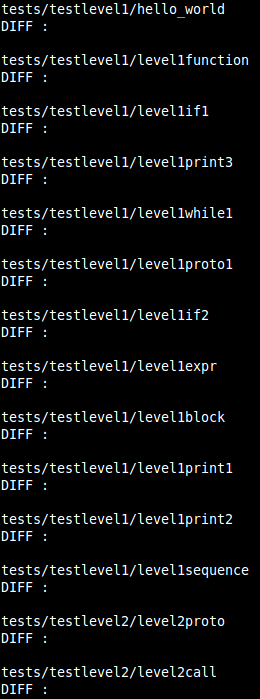
\includegraphics[scale=0.5]{tests}
\caption{
  \textbf{Execution of the tests}.
  If there is a difference between the actual output and the expected output, it appears in the DIFF part.
  This method permits to spot errors easily.}
  \label{fig.test}
\end{figure}


\begin{figure}
\centering
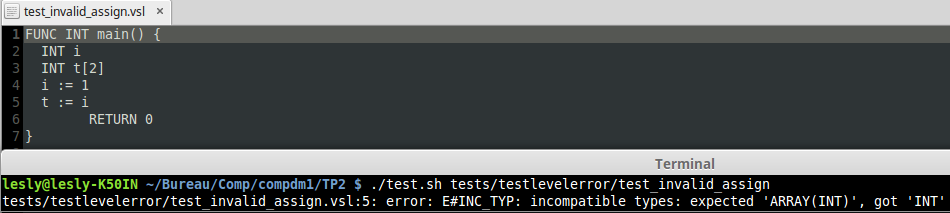
\includegraphics[scale=0.5]{error}
\caption{
  \textbf{Example of error handling}.
  The corresponding file, line, error type and error description appear in the error message.}
  \label{fig.error}
\end{figure}

\begin{figure}
\centering
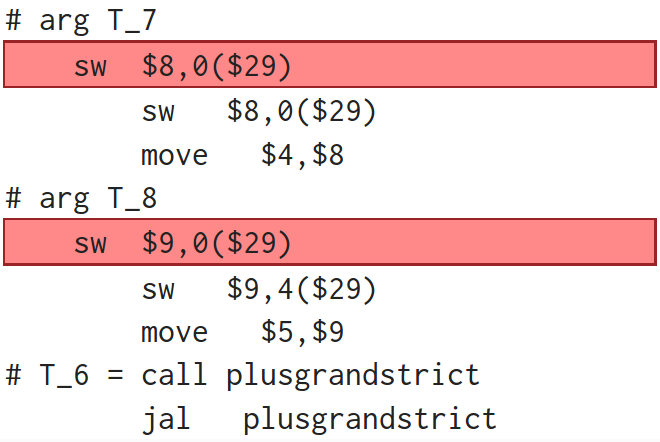
\includegraphics[scale=0.4]{diff}
\caption{
  \textbf{Mips code generated for \textit{tests/monprogramme2.vsl}}.
  The code doesn't work since the first argument is overwritten by the second.
  If the red lines are removed, the program is working.}
  \label{fig.mips}
\end{figure}


\end{document}
